\section{Intermezzo}
\label{sec:intermezzo}

\begin{frame}
	\frametitle{Intermezzo: Network routing}
	\begin{center}
		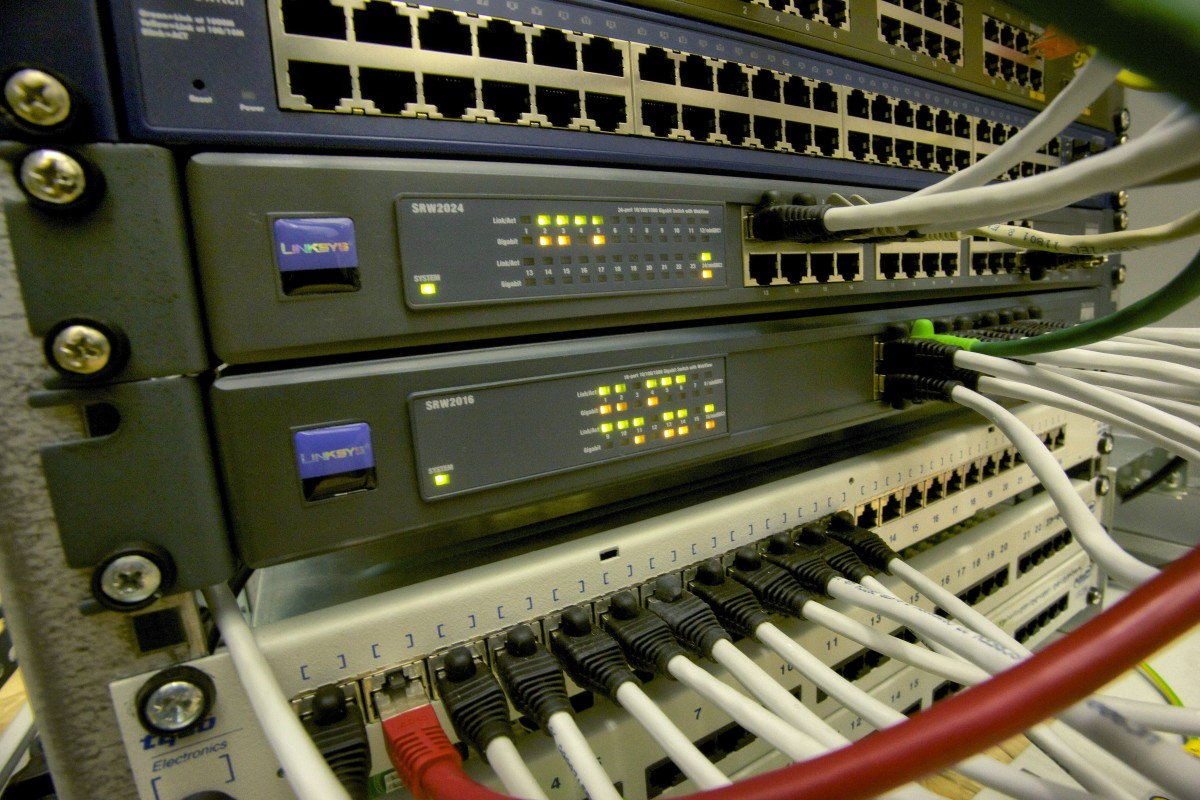
\includegraphics[width=0.7\textwidth]{figures/router.jpg}\\
		\hspace*{15pt}\hbox{\scriptsize Image from: \thinspace{\itshape Pxhere}}
		% https://pxhere.com/en/photo/1116555
	\end{center}
\end{frame}

\begin{frame}
	\frametitle{The Internet}

	\begin{itemize}
		\item The Internet is nothing more than a bunch of:
					\pause
			\begin{itemize}
				\item Wires,
					\pause
				\item \textit{Routers},
					\pause
				\item and \textit{Algorithms}.
			\end{itemize}
		\pause
		\item When sending a message or doing a network request:
			\begin{enumerate}
				\item This enters the \textit{queue} in your Operating System (Windows, Linux, MacOS).
					\pause
				\item This then enters the \textit{queue} in your router.
				\item It passes through another bunch of routers.
					\pause
				\item It enters the \textit{queue} of messages in the OS of the server.
					\pause
				\item It enters the \textit{queue} of open requests in the application at a server.
					\pause
				\item Etc.
			\end{enumerate}
	\end{itemize}
\end{frame}

\begin{frame}
	\frametitle{Traceroute}
	\begin{center}
		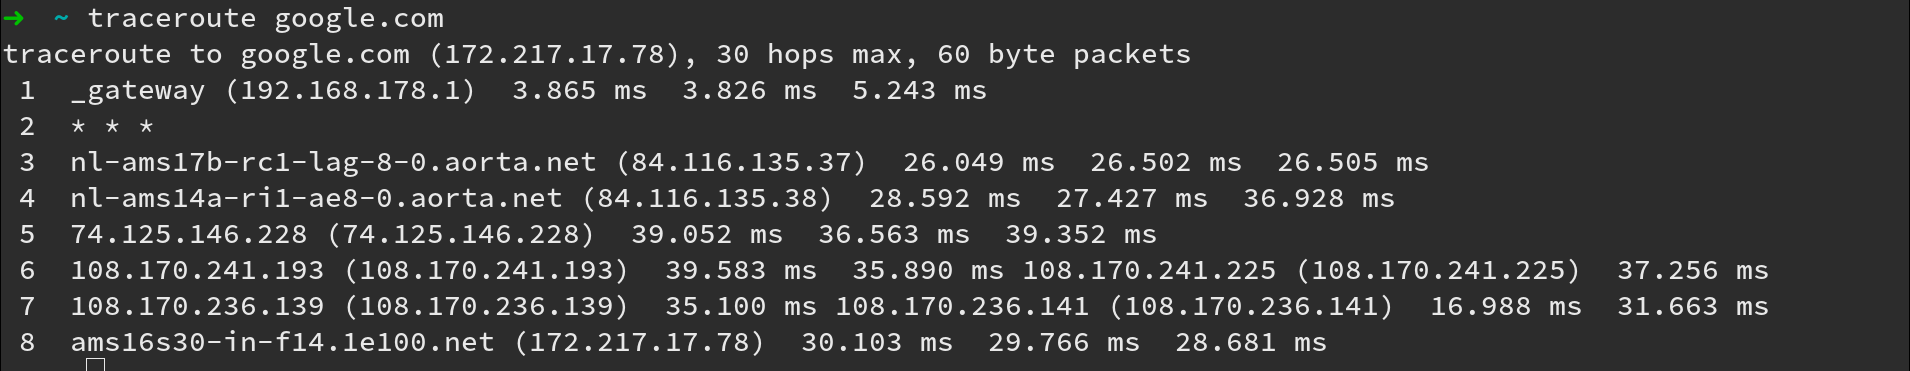
\includegraphics[width=\textwidth]{figures/traceroute.png}\\
		\hspace*{15pt}\hbox{\scriptsize Screenshot by: \thinspace{\itshape Stefan Hugtenburg}}
	\end{center}
		\begin{block}{Traceroute}
			Allows you to see what routers your request came through along the way.\\
			At least 8 here, but notice the massive time difference between 1 and 3...\\
			There are more it seems, but they are \textit{hidden}.
		\end{block}	
\end{frame}

